\documentclass[12pt]{ctexart}

\title{机械设计基础课程设计报告}
\author{欧 宇恒}
\date{\today}
\usepackage{ctex}			%处理中文字体宏包
\usepackage{graphicx}		%处理图片宏包
\usepackage{amsmath}		%处理数学公式宏包	
\usepackage{setspace}		%处理行距宏包
\usepackage[left=1.91cm,right=1.91cm,top=2.54cm,bottom=2.54cm]{geometry}		%编辑页面格式
\usepackage{booktabs}		%处理三线表宏包
\usepackage{color}			%处理颜色宏包
\usepackage{multirow}       %处理合并单元格宏包


\begin{document}	
	\ctexset{
		section={
			name={\S},
			nameformat={\zihao{2}},
			titleformat={\centering\heiti\zihao{2}},
		},
		subsection={
			name={},
			nameformat={\zihao{4}},
			titleformat={\zihao{4}},
		},
	}

    
\begin{titlepage}

    \begin{center}
    % Upper part of the page
    
\includegraphics[width=0.4\textwidth]{./CSU.png}\\[1cm]    
    \textsc{\LARGE Central South University}\\[1.5cm]
    \textsc{\Large Final Week Project}\\[1.5cm]
    % Title
    \textsc{\huge \bfseries 机械设计基础课程设计说明书}\\[1.5cm]
    % Author and supervisor
    \begin{minipage}{0.4\textwidth}
    \begin{flushleft} \large
    \emph{Author:}\\
    OuYuheng
    \end{flushleft}
    \end{minipage}
    \begin{minipage}{0.4\textwidth}
    \begin{flushright} \large
    \emph{Supervisor:} \\
    Dr.Zhou \textsc{Ying}
    \end{flushright}
    \end{minipage}
    
    \vfill
    
    % Bottom of the page
    {\large \today}
    
    \end{center}
    
    \end{titlepage}
%%封面


%%封面 end

\newpage

\tableofcontents

\newpage

\section{轴的设计计算}

\subsection{初算轴的最小直径}

由于本课程设计中采用了齿轮轴的设计方式,兼并了齿轮与轴的两大传动作用,故齿轮与轴的材料选取同一种材料,因此高速齿轮轴材料为 45 号调质钢,低速齿轮轴材料为 45 号钢采用正火处理,轴的最小直径估算公式为:

$$d_{min}=C\sqrt[3]{\frac{P}{n}}$$

其中,$P$为轴的输入功率,$n$为轴的转速,$C$由轴的材料和承载情况确定,依据 [1]P250 表 14-2,初步暂定$C=110$,则有

$$d_{min,1}=110\times \sqrt[3]{\frac{7.2}{301}} = 31.69\text{mm}$$

$$d_{min,2}=110\times \sqrt[3]{\frac{6.77}{98}} = 45.13\text{mm}$$

此时定出的轴径为最小直径,但是由于轴伸处需要切开键槽,需要额外加粗 5\%的轴径,加粗后的轴径为:

$$d_{min,1,plus} = d_{min,1}\times 105\% = 33.28\text{mm}$$

$$d_{min,2,plus} = d_{min,2}\times 105\% = 47.39\text{mm}$$

\begin{figure}[htbp]
    \centering
    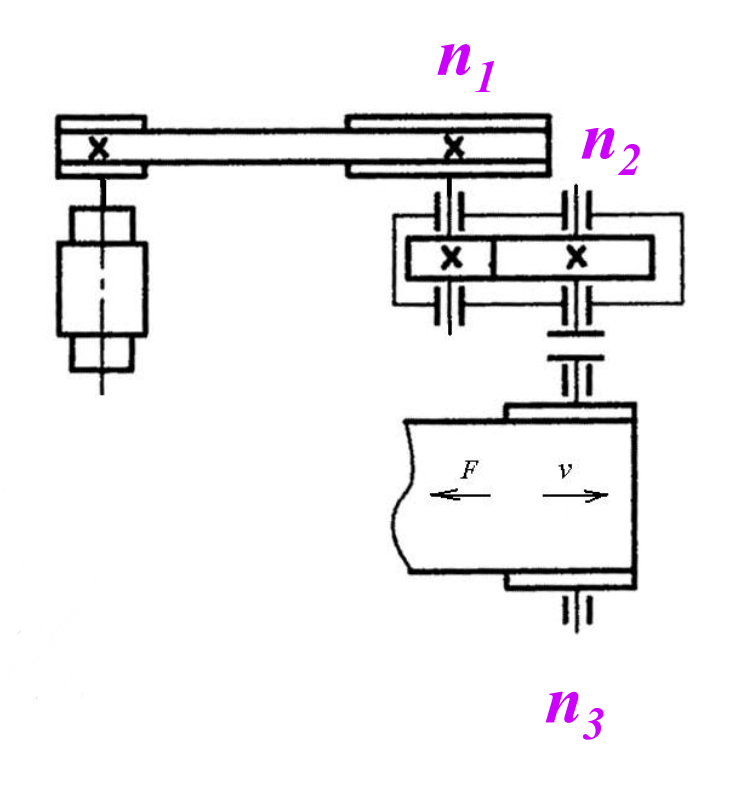
\includegraphics[scale=0.2]{dynamic_argument.png}
    \caption{轴连接示意图}\label{figure7}
\end{figure}

由图\ref{figure7}可以看出,高速轴和低速轴连接的为带轮和联轴器,需要根据标准选择基准直径。高速轴的轴伸连接 V 带轮,需要根据 V 带轮的标准直径选取,查 [3]P227 表 8-15,选取高速轴的基准直径为 $35\text{mm}$;低速轴的轴伸连接联轴器,根据联轴器的标准选取,查 [2]P162 表 17-2,选取低速轴的基准直径为 $50\text{mm}$。

\subsection{带轮的选择}

考虑到本设计选用 B 型带轮,依据大带轮基准直径,通过查 [2]P64 表 9-1,可得带轮的一系列参数如表\ref{table14}所示。

\begin{table}[htbp]
    \centering
    \begin{tabular}{c c}
        \toprule
        参数 & 尺寸值 \\
        \midrule
        V 带型号         & B 型 \\
        $d_d$           & 450 \\
        轮毂长度$l$     & 70 \\
        孔径$d$         & 35 \\
        \bottomrule
    \end{tabular}
    \caption{大带轮选用型号及参数}
    \label{table14}
\end{table}

\subsection{联轴器的选择}

本设计中低速轴与工作机轴相连接,可采用常见的凸缘联轴器,根据公称扭矩,查 [2]P162 表 17-2,主动端选择 J 型轴孔,从动端选择 J1 型轴孔,主从动端轴伸均选用 C 型键槽,因此可选用联轴器型号为:

$$ \text{YL10 联轴器} \frac{JC50\times 84}{J_1C48\times 84}GB5843-86 $$ 

可以得到联轴器各项参数如表\ref{table15}所示。

\begin{table}[htbp]
    \centering
    \begin{tabular}{c c}
        \toprule
        参数 & 参数值 \\
        \midrule
        主动端轴孔长度   & 84 \\
        从动端轴孔长度   & 84 \\
        $L_0$           & 173 \\
        $D$             & 160 \\
        $D_1$          & 130 \\
        螺栓数量        & 4* (铰制孔连接)\\
        螺栓直径        & M12\\
        \bottomrule
    \end{tabular}
    \caption{联轴器参数}
    \label{table15}
\end{table}

\subsection{键的选择}

本项目中高低速轴与齿轮轮毂连接处选用 A 型平键作为键连接方式,轴伸与带轮、联轴器连接处选用 C 型平键作为键连接方式,根据轴的直径,查 [2]P140 表 14-1 可得键的型号见表\ref{table16}所示。

\begin{table}[htbp]
    \centering
    \begin{tabular}{c c c c}
        \toprule
        轴段 & 键的类型 & 键的公称尺寸  & 键长/mm \\
        \midrule
        高速轴与齿轮轮毂连接   & A 型 & $14\times 9$    & 111\\
        低速轴与齿轮轮毂连接   & A 型 & $20\times 12$   & 101\\
        高速轴与带轮连接      & C 型  & $10\times 8$     & 45\\
        低速轴与联轴器连接    & C 型  &  $14 \times 9$    & 65\\
        \bottomrule
    \end{tabular}
    \caption{各个轴段选取的键连接型号}
    \label{table16}
\end{table}



\subsection{确定各轴段直径}

接下来需要确定各轴段直径,各轴段序号标注如图\ref{figure8}所示:

\begin{figure}[htbp]
    \centering
    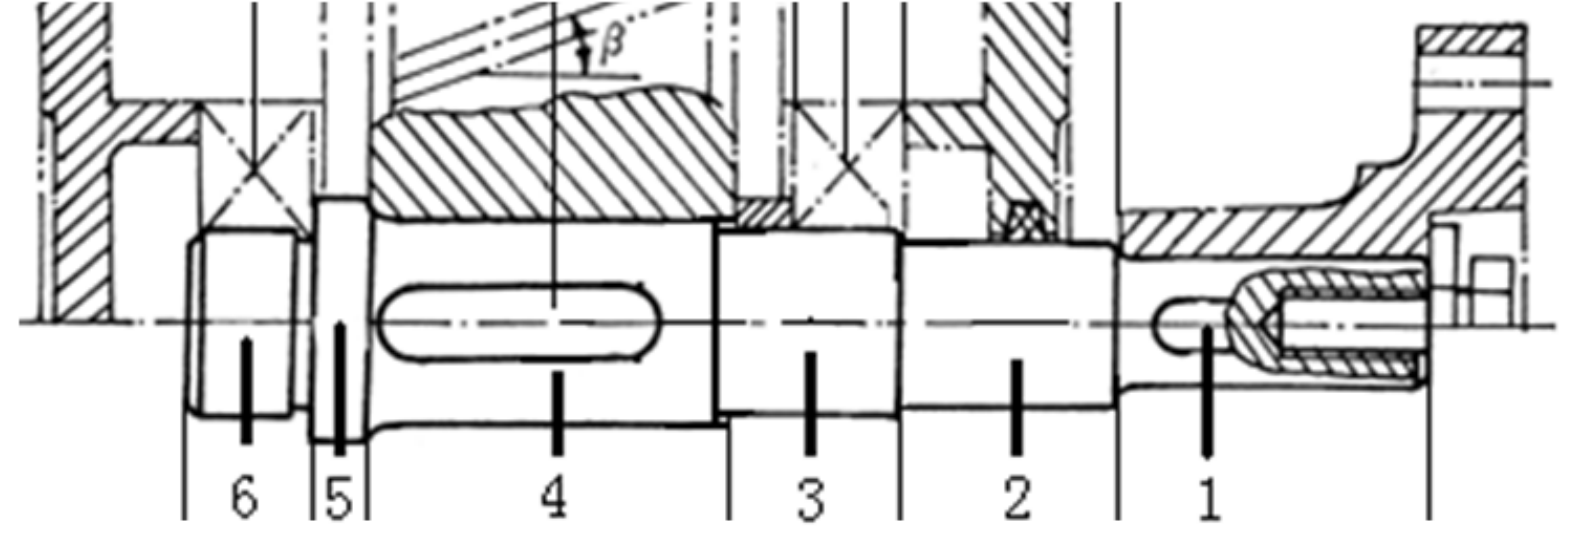
\includegraphics[scale=0.2]{roller.png}
    \caption{轴段序号标注示意图}\label{figure8}
\end{figure}

其中,轴段 1 的直径为前期计算已经确定的最小基准轴径;轴段 2 则根据密封圈标准件的基准直径确定,且要求 D2 较 D1 大于 $6\sim 10 \text{mm}$ 通过查表 [2] P158 表 16-9 可得;轴段 3 的直径较 D2 大于$1\sim 5\text{mm}$且需要为 5 的倍数,以此匹配轴承的需要;轴段 4 需要与大齿轮匹配,需要查 [2]P117 表 11-2 查出大齿轮的基准直径;轴段 5 有定位要求,需要较 D4 大 $6 \sim 10 \text{mm}$;由于同轴上的两轴承内外径大小一致,轴段 6 与轴段 3 直径相等,但同时需要满足轴承安装高度的要求(如表\ref{table10}所示),考虑到在高速轴中,轴承安装高度与 D5 矛盾,需要将 D5 设计成两段阶梯的轴肩,设计出的各轴段直径设计尺寸如表\ref{table9}所示。

查轴承的安装尺寸,查 [2]P144 表 15-3,得到高速轴与低速轴选用轴承与相关参数如表\ref{table10}所示。
\begin{table}[htbp]
    \centering
    \begin{tabular}{c c c}
        \toprule
        型号及参数 & 高速轴& 低速轴\\
        \midrule
        轴承型号 & 6309(新标准) & 6313(新标准) \\
        内径$d$/mm & 45 & 65 \\
        外径$D$/mm & 100 & 140 \\
        安装尺寸/mm & 54 & 77 \\
        轴承宽度/mm & 25 & 33 \\
        \bottomrule
    \end{tabular}
    \caption{轴承选用型号及参数}
    \label{table10}
\end{table}


\begin{table}[htbp]
    \centering
    \begin{tabular}{c c c}
        \toprule
        直径 & 轴 1& 低速轴\\
        \midrule
        D1/mm & 35 & 50 \\
        D2/mm & 42 & 60 \\
        D3/mm & 45 & 65 \\
        D4/mm & 50 & 67 \\
        D5/mm & 54(左),56(右) & 77 \\
        D6/mm & 45 & 65 \\
        \bottomrule
    \end{tabular}
    \caption{各轴段直径设计尺寸}
    \label{table9}
\end{table}

\subsection{润滑方式选择}

\subsubsection{轴承的润滑方式选择}

本设计通过速度因数$dn$值对轴承润滑方式选择,根据 [1]P289 图 16-11 选择润滑方式。

通过计算,本设计中各个轴承的$dn$值如表\ref{table12}所示:

\begin{table}[htbp]
    \centering
    \begin{tabular}{c c c c}
        \toprule
        轴 & 轴承内径/mm & 转速/(r/min) & 速度因数/(r·mm/min)\\
        \midrule
        高速轴 & 45 & 301 & 13545 \\
        低速轴 & 65 & 98  & 6370  \\
        \bottomrule
    \end{tabular}
    \caption{各轴承速度因数值}
    \label{table12}
\end{table}

由于高速轴和低速轴的速度因数均$<(2\sim 3)\times 10^5 \text{mm·r/min}$,故均选用脂润滑。

\subsubsection{齿轮的润滑方式选择}

由于本设计中齿轮的轮系速度$v<12m/s$,故齿轮的润滑方式选择油润滑。

\subsection{轴段长度确定}

各个轴段长度需要根据画图确定,各段长度确定方法确定如下。

\begin{itemize}
    \item 
\end{itemize}

\section{减速器箱体设计}
\subsection{铸铁减速器箱体结构尺寸}

查阅 [2]P17 表 3-1 对减速器的箱体结构尺寸进行设计,其中螺纹直径查 [2]P126 表 13-1。

\begin{table}[htbp]
    \centering
    \begin{tabular}{c c l c}
        \toprule
        \textbf{名称} & \textbf{符号} & \textbf{尺寸计算公式} & \textbf{设计尺寸/mm} \\
        \midrule
        箱座壁厚                      & $\delta$    & $\delta = max\{0.025a+1,8\}$    & 8 \\
        箱盖壁厚                      & $\delta_1$  & $\delta_1 = max\{0.02a+1,8\}$   & 8 \\
        \multirow{3}{*}{箱体凸缘厚度} & 箱座$b$      & $b=1.5\delta $                  & 12\\
                                     & 箱盖$b_1$    & $b_1 =1.5\delta_1$              & 12\\
                                     & 箱底座$b_2$  & $b_2 =2.5\delta$                & 20 \\
        \multirow{2}{*}{加强肋厚}     & 箱座$m$      & $m=0.85\delta $                & 7 \\
                                     & 箱盖$m_1$    & $m_1=0.85\delta_1$              & 7\\
        地脚螺钉直径                  & $d_f$        & $d_f=0.036a+12$                 & 4 \\
        轴承旁联接螺栓直径             & $d_1$        & $d_1=0.75d_f$                  & 18\\
        箱盖、箱座联接螺栓直径         & $d_2$        & $d_2=(0.5\sim 0.6)d_f$         & 12 \\
        轴承盖螺钉直径                & $d_3$        & \multirow{2}{*}{查 [2]P77 表 9-9} & 8(轴 1),10(轴 2) \\
        轴承盖螺钉数目                & $n$          &                                 & 4(轴 1),6(轴 2)\\
        轴承盖(轴承座端面)外径       & $D_2$        & $D_2=D+5d_3$                    & 140(轴 1),190(轴 2) \\
        轴承两侧联接螺栓间距离         & $s$          & $s\approx D_2$                  & 140(轴 1),190(轴 2)\\
        观察孔盖螺钉直径              & $d_4$        & $d_2=(0.3\sim 0.4)d_f$          & 8 \\
        $d_f$至箱外壁距离             & $C_{1,min}$  & \multirow{6}{*}{查 [2]P17 表 3-1}  & 30\\
        $d_f$至凸缘外缘距离           & $C_{2,min}$  & & 26\\
        $d_1$至箱外壁距离             & $C_{1,min}$  & & 24\\
        $d_1$至凸缘外缘距离           & $C_{2,min}$  & & 22\\
        $d_2$至箱外壁距离             & $C_{1,min}$  & & 18\\
        $d_2$至凸缘外缘距离           & $C_{2,min}$  & & 16\\

         \bottomrule
    \end{tabular}
    \caption{减速器箱体结构设计尺寸}
    \label{table11}
\end{table}

\subsection{减速器零件的位置尺寸}

接下来根据 [2]P24 表 4-1 对减速器零件的位置尺寸进行确定,经过计算后得到的结果如表\ref{table13}所示。

\begin{table}[htbp]
    \centering
    \begin{tabular}{c c c c}
        \toprule
        名称 & 符号 & 设计尺寸/mm \\
        \midrule
        齿轮顶圆至箱体内壁的距离     & $\Delta_1$ & 10 \\
        齿轮端面至箱体内壁的距离     & $\Delta_2$ & 10 \\
        轴承端面至箱体内壁的距离     & $\Delta_3$ & 11 \\
        齿轮顶圆至轴表面距离         & $\Delta_5$ & 12 \\
        大齿轮齿顶圆至箱体内壁的距离  & $\Delta_6$ & 40 \\
        箱底至箱底内壁的距离         & $\Delta_7$ & 20 \\
        减速器中心高                & $H$        & 238 \\
        箱体内壁至轴承座孔端面的距离  & $L_1$      & 60 \\
        轴承端盖凸缘厚度            & $e$         & 10(轴 1),12(轴 2)\\
        
        \bottomrule
    \end{tabular}
    \caption{减速器零件的位置设计尺寸}
    \label{table13}
\end{table}

\newpage

\section{参考文献}

[1] 杨可桢,程光蕴。机械设计基础。6 版。北京:高等教育出版社,1979.

[2] 王昆。机械设计基础课程设计。北京:高等教育出版社,1995.

[3] 唐金松。简明机械设计手册。3 版。上海:上海科学技术出版社,1992.



\end{document}